\documentclass[10pt,a4paper]{article}

\usepackage{fontspec}
\setmainfont{Public Sans}[
  Path           = ./fonts/,
  Extension      = .ttf,
  BoldFont       = PublicSans-Bold,
  ItalicFont     = PublicSans-Italic,
  BoldItalicFont = PublicSans-BoldItalic
]

\usepackage{geometry}
\usepackage{xcolor}
\usepackage{enumitem}
\usepackage{titlesec}
\usepackage{hyperref}
\usepackage{graphicx}
\usepackage{tikz}
\usepackage{parskip}

\geometry{top=1.2cm,bottom=1.2cm,left=1.1cm,right=1.1cm,columnsep=0.8cm}

\hypersetup{colorlinks=true, urlcolor=black, linkcolor=black}

\definecolor{lightgray}{RGB}{180,180,180}
\definecolor{sectioncolor}{RGB}{30,30,30}

\titleformat{\section}
  {\normalfont\bfseries\large\color{sectioncolor}}
  {}{0em}{}[\vspace{-4pt}\color{lightgray}\rule{\linewidth}{0.4pt}\vspace{2pt}]

\titlespacing{\section}{0pt}{10pt}{4pt}

\linespread{1.04}
\setlength{\parindent}{0pt}
\setlength{\parskip}{2pt}

\setlist[itemize]{leftmargin=1em,itemsep=1pt,topsep=2pt,parsep=0pt,label=\textbullet}

\newcommand{\entry}[3]{%
  \textbf{#1} \hfill \textit{\small #2}\\
  \small #3\par\vspace{8pt}
}

\newcommand{\entryshort}[2]{%
  \textbf{#1} \hfill \textit{\small #2}\par
}

\pagestyle{empty}

\begin{document}

%% ─── HEADER ──────────────────────────────────────────────────────────────────
\begin{minipage}[t]{0.18\linewidth}
  \vspace{0pt}
  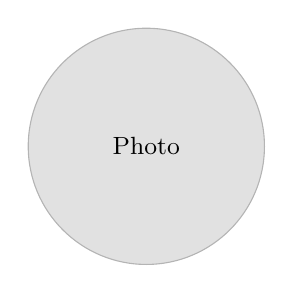
\begin{tikzpicture}
    \draw[fill=lightgray!40, draw=lightgray] (0,0) circle (1.5cm);
    \node at (0,0) {\small Photo};
  \end{tikzpicture}
\end{minipage}%
\hfill
\begin{minipage}[t]{0.79\linewidth}
  \vspace{0pt}
  {\fontsize{28}{32}\selectfont\textbf{Maxandre Berson-Lefuel}}\\[6pt]
  Étudiant ingénieur à l'EFREI en informatique spécialisé en réseaux et sécurité, je recherche une alternance (année 2026-2027, 1sem/1sem). Je maîtrise également le développement fullstack ainsi que le management et la gestion de projets grâce à ma formation DUT.
\end{minipage}

\vspace{8pt}

%% ─── TWO-COLUMN BODY ─────────────────────────────────────────────────────────
\begin{minipage}[t]{0.30\linewidth}
\vspace{0pt}

(+33) 07 68 66 90 10\\
\href{mailto:maxandre@synae.dev}{maxandre@synae.dev}\\
Marcoussis (91460)\\
Permis B\\
\href{https://www.linkedin.com/in/maxandre-bl/}{linkedin.com/in/maxandre-bl/}\\[4pt]
\textbf{Portfolio} : \href{https://maxx-bl.github.io/}{maxx-bl.github.io/}

\vspace{2pt}
\color{lightgray}\rule{\linewidth}{0.4pt}
\color{black}

\section*{COMPÉTENCES}

\begin{itemize}
  \item \textbf{Développement web :}\\
    JavaScript, HTML, CSS, PHP
  \item \textbf{Développement logiciel :}\\
    Python, Java, C\#, C++, C
  \item \textbf{Base de données :}\\
    SQL, MySQL, SQLite, Oracle, UML, Looping, Mocodo
  \item \textbf{Outils :}\\
    Flutter, React Native, Unity, Godot, Docker
  \item \textbf{GIT :}\\
    GitHub, GitLab, Bash + GUI
  \item \textbf{Sécurité \& Réseaux :}\\
    Wireshark, Nmap, Hydra, MetaSploit, TCP/IP/UDP, SSH, Firewall
\end{itemize}

\section*{QUALITÉS}

\begin{itemize}
  \item \textbf{Travail d'équipe :} Collaboration avec graphistes et développeurs
  \item \textbf{Polyvalence :} Web, Logiciel, Mobile
  \item \textbf{Pédagogie :} Cours particuliers à domicile et distanciel
  \item \textbf{Adaptation :} Apprentissage rapide de technologies / frameworks
\end{itemize}

\section*{LANGUES}

\begin{itemize}
  \item \textbf{Français} (langue maternelle)
  \item \textbf{Anglais} (niveau C1)
\end{itemize}

\section*{LOISIRS}

\begin{itemize}
  \item \textbf{Musique :} Piano (classique, pop, indé) depuis 2012, Composition (FL Studio)
  \item \textbf{Sport :} Callisthénie
\end{itemize}

\end{minipage}%
\hfill
\begin{minipage}[t]{0.67\linewidth}
\vspace{0pt}

\section*{PROJETS INFORMATIQUES}

\entry{Réseau social « Glyphe »}{2025 / 2026}{Développement d'une application mobile avec Flutter, communicante avec une base de données Firebase. Système de messagerie, followers et de posts.}

\entry{Code Game Jam IUT Montpellier-Sète}{2025 et 2026}{Conception de jeux vidéo (équipe de 6 personnes, 30h) sur Godot. Jeu de rythme musical en C\# (2025) et clicker game en GDScript (2026).}

\entry{Site internet Ethix IT et Ethix Marine}{2023}{Création de sites internet pour deux sociétés commerciales, en utilisant HTML, CSS et JavaScript.}

\entry{Jeu vidéo mobile « RockingBall »}{2023 / 2024}{Développement sur Godot (C\#) et publication d'un jeu vidéo sur Android, réalisé en collaboration avec un graphiste.}

\entry{Jeux multijoueurs « SpaceY » et « Solanum RPG »}{2022 / 2024}{Conception de deux jeux multijoueurs, Godot et utilisation de l'API discord.js et node.js.}

\vspace{14pt}
\section*{EXPÉRIENCES PROFESSIONNELLES}

\entry{Développeur C\# chez Simutech uae}{2026}{Développement \& conception d'une application de post traitement de données/mesures (tests API, analyse de flux).}

\entry{Tuteur chez IUT Paris-Saclay}{2025 / 2026}{Cours de soutien en C++ et système Linux aux élèves de première année.}

\entry{Enseignant particulier chez À domicile / distanciel}{2024 / 2026}{Soutien scolaire en Mathématiques, Informatique (élèves lycée), aide aux devoirs / babysitting (élèves primaire).}

\vspace{14pt}
\section*{FORMATIONS}

\entry{EFREI, Majeure réseaux \& sécurité}{2026 / 2029}{Cycle ingénieur, majeure réseaux \& sécurité.}

\entry{IUT d'Orsay, DUT Informatique}{2024 / 2026}{Section anglophone, spécialité cybersécurité \& réseaux, option mathématiques ingénieur.}

\entry{EPITA, Prépa intégrée}{2023 / 2024}{Première année de programme préparatoire intégré.}

\entry{Lycée Institution du Sacré-Cœur / Essouriau, Baccalauréat général}{2020 / 2023}{Mention bien, spécialités Mathématiques et NSI.}

\entry{Secourisme, PSC1}{2020}{Obtention du brevet de secourisme PSC1.}

\end{minipage}

\end{document}
